\subsection{Limitazioni: Gestione dei driver audio}\label{subsec:mischeWilhelm}
L'obiettivo di questa sottosezione è quello di dimostrare come, all'interno dello
stesso sistema operativo messo a disposizione da Google, siano presenti 
forti limitazioni architetturali, che impongono la necessità di applicare
estensioni allo stesso sistema operativo. 
\bigskip

Per capire meglio il meccanismo di lettura da \texttt{\small AudioRecorder}, debbo descrivere
inizialmente il meccanismo di inizializzazione della procedura. Partendo quindi 
dalla funzione della libreria \texttt{\small wilhelm} \texttt{\small android\_audioRecorder\_realize},
 si effettua l'invocazione del metodo \texttt{\small set} dell'oggetto \texttt{\small AudioRecord}
definito dall'omonimo file presente all'interno del percorso:
\begin{center}
\texttt{\small \AOSP/frameworks/av/media/libmedia}
\end{center}
Accedendo al codice sorgente, possiamo notare come non venga passato un 
\textit{session Id} (o meglio come venga implicitamente passato il valore 0, allo scopo di generarne
uno automaticamente con il metodo \texttt{\small AudioSystem::newAudioSessionId()})
e come venga passato come argomento \texttt{\small cbf} la funzione 
\texttt{\small audioRecorder\_callback} fornita da \texttt{\small wilhelm}, in modo da fornire alla libreria il 
\textit{sampling} audio ottenuto.

Analizzando ora il metodo \texttt{\small AudioSystem::getInput()}, possiamo notare come
venga ad esso passato un numero nuovo di sessione, e di come si invochi il
metodo \texttt{\small getInput} di \texttt{\small AudioPolicyService} dopo aver
richiesto al Binder un \textit{proxy} per instaurare la comunicazione con detto \textit{service}.

Dopo aver osservato che questo \textit{service}, come da implementazione all'interno
del file:
\begin{center}
\texttt{\small \AOSP/frameworks/av/services/audioflinger/AudioPolicyService.cpp/h}
\end{center} 
effettua l'estensione della classe \texttt{\small BnAudioPolicyService}, si può notare
come, nel metodo ivi definito, l'operazione basilare sia quella di ottenere 
il puntatore alla funzione di ottenimento dell'input dalla scheda audio.

	Analizzando quindi la procedura \texttt{\small set} della
	classe \texttt{\small AudioRecorder}, si effettua l'invocazione del metodo
	\texttt{\small openRecord\_l}, dove ancora una volta 
	si ottiene con il metodo \texttt{\small AudioSystem::get\_audio\_flinger()}
	un'istanza del proxy \texttt{\small BpBinder} per comunicare con il \textit{service}
	\texttt{\small AudioFlinger}.
	
	Come posso osservare dall'invocazione del metodo \texttt{\small checkRecordThread\_l},
	è necessario che si verifichi la creazione di un \texttt{\small RecordThread}.
Tuttavia non è immediato mostrare come sia possibile inserire tale thread.
\textit{Voglio quindi mostrare come, oltre all'utilizzo del Binder, anche i metodi
di classi possano mettere in comunicazione diversi oggetti tramite puntatori 
a funzione definiti all'interno di strutture dati C, che in particolare
contengono puntatori a funzioni che consentono l'IPC tramite Binder}.
\medskip

Analizzo quindi il costruttore della classe \texttt{\small AudioPolicyService}.
Per quanto concerne l'inizializzazione, devo far ancora riferimento al \textit{server}
principale, ovvero il \texttt{\small mediaserver} di cui si è già discusso il codice.

Faccio riferimento alla figura \vref{fig:functioncallAudio} per esporre in 
un modo più chiaro i meccanismi di chiamata di quanto non sia possibile fare
a parole, col rischio di perdere l'idea del susseguirsi delle chiamate a funzione.
\textit{In particolare il meccanismo di apertura del modulo mette in luce una potenziale
fragilità del sistema: sarebbe infatti sufficiente cambiare il modulo \texttt{\small .so} per 
cambiare il comportamento delle funzioni che seguono}.

\begin{figure}[thp]
\begin{cpp}[mathescape=true]
struct audio_policy_service_ops aps_ops = {
  ...
  open_input : aps_open_input
  $\drsh$ AudioSystem::get_audio_flinger()->openInput(...)
    $\drsh$ AudioFlinger::openInput(...)
      $\drsh$ mRecordThreads.add(id,new RecordThread(this,...));
  ...
  open_input_on_module : aps_open_input_on_module 
  $\drsh$ AudioSystem::get_audio_flinger()->openInput(...)
    $\drsh$ ...
} [./frameworks/av/services/audioflinger/AudioPolicyService.cpp]

AudioPolicyService::initiate() [AudioFlinger]
$\drsh$ AudioPolicyService::AudioPolicyService() 
  $\drsh$ {
      hw_get_module(AUDIO_POLICY_HARDWARE_MODULE_ID,&module);
      $\drsh$ AUDIO_POLICY_HARDWARE_MODULE_ID = audio_policy [audio_policy.h]
        Il nome del binario dalla compilazione di hardware/libhardware_legacy/audio
        $\drsh$ hw_get_module [hardware.c]
          $\drsh$  hw_get_module_by_class
            $\drsh$ Caricamento dei moduli di nome AUDIO_POLICY_HARDWARE_MODULE_ID tramite dlopen
  
       audio_policy_dev_open(module,&mpAudioPolicyDev) [definito in audio_policy.h]
       $\drsh$ module->methods->open(module,"policy",...) 
         dove open = default_ap_dev_open [audio_policy.c]
       
       mpAudioPolicyDev->create_audio_policy(mpAudioPolicyDev,&aps_ops,this,...);
         $\drsh$ create_legacy_ap(mpAudioPolicyDev,&aps_ops,this,..) [audio_policy_hal.cpp]
         {
           lap->service_client = new AudioPolicyCompatClient(aps_ops, service) [AudioPolicyCompatClient.cpp]
           $\drsh$ mServiceOps:=&aps_ops  mService:=this
           lap->apm = createAudioPolicyManager(lap->service_client) 
           $\drsh$ AudioPolicyManager(lap->service_client) [AudioPolicyManager.cpp] sottoclasse di:
             $\drsh$ AudioPolicyManagerBase::AudioPolicyManagerBase(lap->service_client)
               $\drsh$ mpClientInterface = lap->service_client
         }
  }
\end{cpp}
\caption{\textit{Inizializzazione delle strutture dati C di collegamento}.}
\label{fig:functioncallAudio}
\end{figure}

Ritornando quindi per un momento all'invocazione del metodo\\ \texttt{\small AudioPolicyService::getInput},
otteniamo la sequenza di invocazioni illustrata nella Figura \vref{fig:functioncallThreadAudio},
le quali consentono la creazione di un nuovo thread per la registrazione, tramite
l'apertura di uno \textit{stream} audio in entrata dal driver, non mostrato
per motivi di brevità e ad ogni modo osservabile all'interno del metodo \texttt{\small AudioFlinger::openInput()},
e comunque ottenibile tramite la funzione \texttt{\small mInput} del thread
in questione.

\begin{figure}[thp]
\begin{cpp}[mathescape=tre]
AudioPolicyService::getInput()
$\drsh$ mpAudioPolicy->get_input()
  $\drsh$ lap->apm->getInput() [audio_policy_hal.cpp] (ovvero AudioPolicyManagerBase)
    $\drsh$ AudioPolicyManagerBase::getInput() 
      $\drsh$ mpClientInterface->openInput() [AudioPolicyManagerBase.cpp]
        $\drsh$ AudioPolicyCompatClient::openInput() 
          $\drsh$ mServiceOps->open_input_on_module() [AudioPolicyCompatClient.cpp]
           $\drsh$  aps_open_input_on_module() [AudioPolicyService.cpp]
             $\drsh$ AudioFlinger::openInput() 
              $\drsh$ mRecordThreads.add(id,new RecordThread(this,...))
\end{cpp}
\caption{\textit{Inizializzazione nascosta del thread di registrazione}.}
\label{fig:functioncallThreadAudio}
\end{figure}

Posso quindi palesare con la Figura \vref{fig:tantorumorepernulla} come questo
meccanismo di chiamata si riassuma nella chiamata ad \texttt{\small openInput()},
che tuttavia poteva essere già effettuata a livello di \texttt{\small AudioPolicyService}
tramite l'utilizzo diretto del meccanismo di IPC. 
Si può inoltre notare dal codice sorgente di \texttt{\small AudioFlinger.cpp}
come la creazione di tale \textit{stream} sia assolutamente indipendente dal
chiamante, in quanto non viene conservata alcuna informazione in merito.

In questo modo ho finito di dettagliare la procedura di inizializzazione, e
di come si utilizzino librerie di basso livello per celare il collegamento
tra di esse tramite Binder.
\begin{figure}[thp]
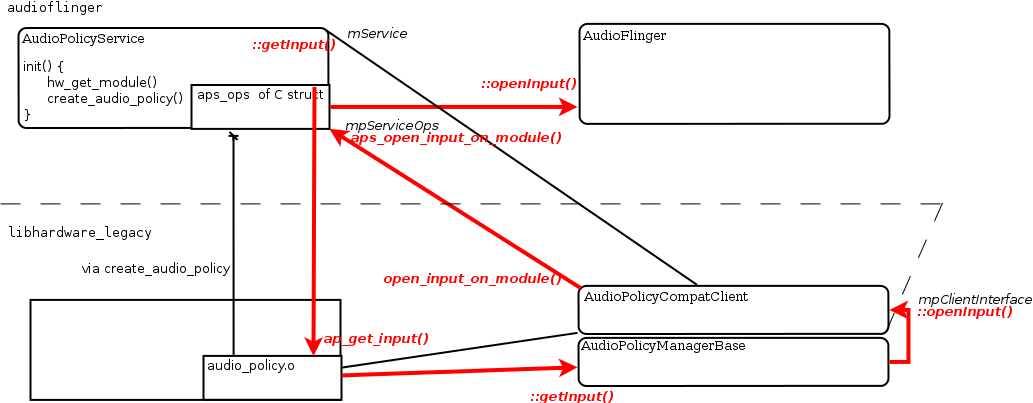
\includegraphics[scale=0.5]{img/modelio/cstructcall.png}
\caption{\textit{Inizializzazione nascosta del thread di registrazione}.}
\label{fig:tantorumorepernulla}
\end{figure}

Ritornando all'invocazione del metodo \texttt{\small AudioFlinger::openRecord}, 
possiamo ora vedere come il thread ottenuto dalla funzione \texttt{checkRecordThread\_l}
sia in particolare il risultato delle complesse interazioni mostrate sopra.
\medskip 


Tramite l'invocazione del metodo \texttt{\small registerPid\_l} si provoca, se non
già esistente, un istanza di un oggetto \texttt{\small Client}, il quale tramite
l'istanziazione di un \texttt{\small MemoryDealer}, ottiene della memoria allocata
dal servizio \textit{ashmem} in modo che questa possa essere condivisa tra processi
differenti.

Eseguendo quindi sul suddetto thread il metodo \texttt{\small createRecordTrack} che,
dopo una serie di invocazione di metodi, effettua l'inizializzazione della
memoria precedentemente allocata: l'oggetto ottenuto come risultato di questa
invocazione sarà utilizzato come argomento del costruttore dell'oggetto di
tipo \texttt{\small RecordHandle}, che si preoccuperà in seguito della lettura da
interfaccia.


Concludendo quindi la procedura di inizializzazione tramite invocazione del 
metodo \texttt{\small set()}, dopo aver invocato \texttt{\small AudioSystem::getInput()}
e \texttt{\small openRecord\_l} nella classe \texttt{\small AudioRecord}, si procede
alla creazione di un'istanza di oggetto \texttt{\small ClientRecordThread},
associata alla variabile \texttt{\small mClientRecordThread}.
\bigskip

Proseguo ora l'analisi con l'invocazione del metodo \texttt{\small start()} 
sull'oggetto \texttt{mAudioRecord} a livello di \texttt{\small wilhelm}, invocato
all'interno della funzione \texttt{\small SetRecordState}; come posso notare
dal codice di \texttt{\small AudioRecord.cpp}, in questo metodo vengono iniziati
sia il thread di lettura del client, sia quello in lettura dal driver audio:
si può quindi notare da codice come questi comunichino tramite l'utilizzo
dell'area di memoria allocata tramite il servizio \textit{ashmem}. Il meccanismo
di Figura \subref{subfig:threadallavoro} \vref{fig:recconclusion}.

Ho messo in questo modo in evidenza come, il codice sopra definito, non consenta
minimamente una politica di caching per il livello di
applicazioni native, allo scopo di far attingere ai dati i 
registratori. Ad ulteriore riprova è il messaggio di errore fornito dall'esecuzione
di due client \texttt{\small pjsua} e riscontrabile all'interno del LogCat:
\begin{bash}
W/AudioRecord(  963): obtainBuffer timed out (is the CPU pegged?) user=00001080, server=00001080
W/AudioTrack(  963): obtainBuffer timed out (is the CPU pegged?) 0x15e16d8 name=0x2user=000011ff, server=000009bf
W/AudioTrack(  963): obtainBuffer timed out (is the CPU pegged?) 0x15e16d8 name=0x2user=000011ff, server=000009bf
\end{bash}
Questo messaggio è causato dalla mancanza di frame in lettura, come riscontrabile
all'interno dalla \texttt{\small while (framesReady==0)} all'interno del metodo\\
\texttt{\small AudioRecord::obtainBuffer} usato dal servizio in lettura sull'area
di memoria condivisa con l'altro Thread, dopo un prefissato tempo d'attesa. Ciò implica che uno dei due thread non
farà mai in tempo ad accedere alle informazioni che pervengono dal microfono
del dispositivo, rimanendo sempre quindi in attesa di ricevere ulteriori informazioni.

Posso di fatti ampliare la gerarchia di Android con la Figura \subref{subfig:gennatserv}
\vref{fig:recconclusion}, mostrando anche l'interazione tra \textit{service} nativi ed applicazioni
native.

\begin{figure}[!h]
\centering
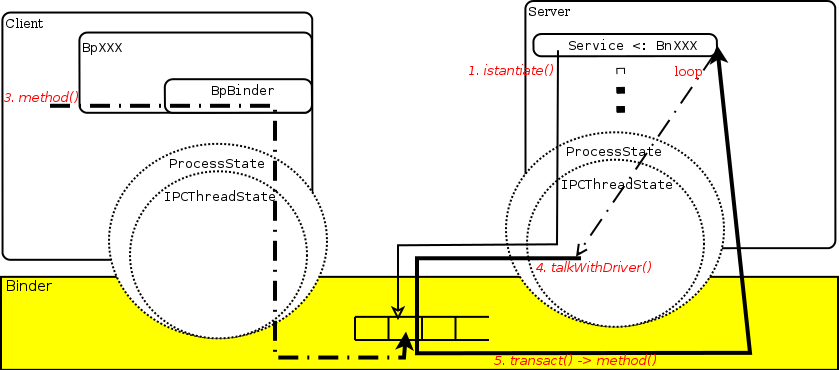
\includegraphics[scale=0.5]{img/modelio/complintrmodelio.png}\\
\caption{\textit{Visione d'insieme di interazione tra client e server}.}
\label{fig:ipcbindconclusion}
\end{figure}

\begin{figure}[p]
\centering
\subfloat[][\textit{Interazione tra i thread di lettura dal driver e di callback verso la libreria wilhelm}.]{\label{subfig:threadallavoro}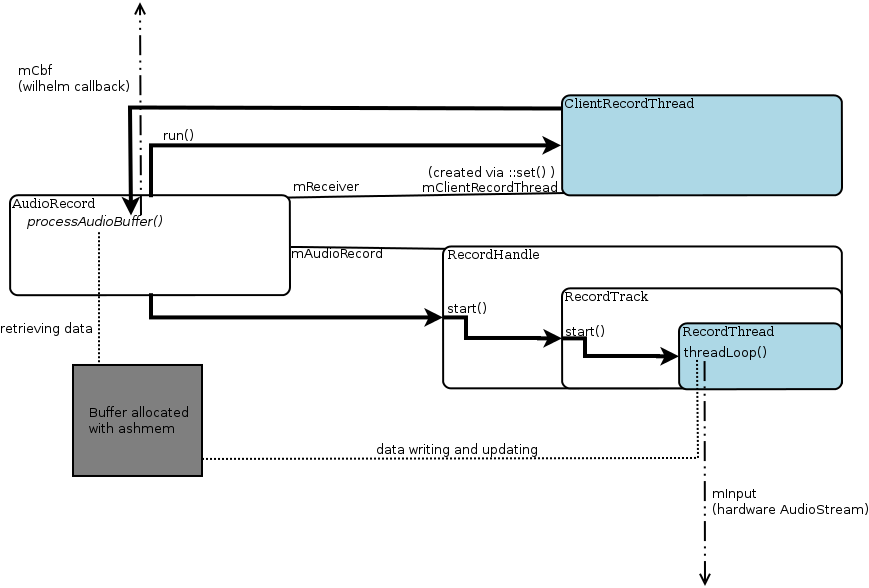
\includegraphics[scale=0.5]{img/modelio/threadbuffer.png}}\\
\subfloat[][\textit{Ampliamento dell'architettura Android con i Native Service}.]{\label{subfig:gennatserv}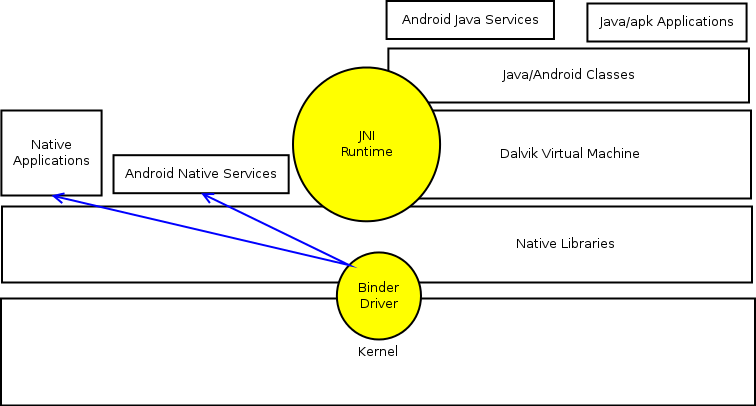
\includegraphics[scale=0.6]{img/modelio/conclus_servandroicpp.png}}\\
\caption{Conclusioni sui metodi di interazione.}
\label{fig:recconclusion}
\end{figure}

Posso inoltre riassumere con la Figura \vref{fig:ipcbindconclusion} l'interazione
che avviene tra \textit{client} e \textit{service} contenuto all'interno di un processo
\textit{server}.


